% Introducción
\begin{frame}{Polígonos Ortogonales.} %%Otra forma (más corta) de poner el título a la diapositiva
  Un polígono simple en el plano se llama ortogonal si sus aristas son paralelas a los
  ejes coordenados.
  
  \begin{figure}
    \centering
    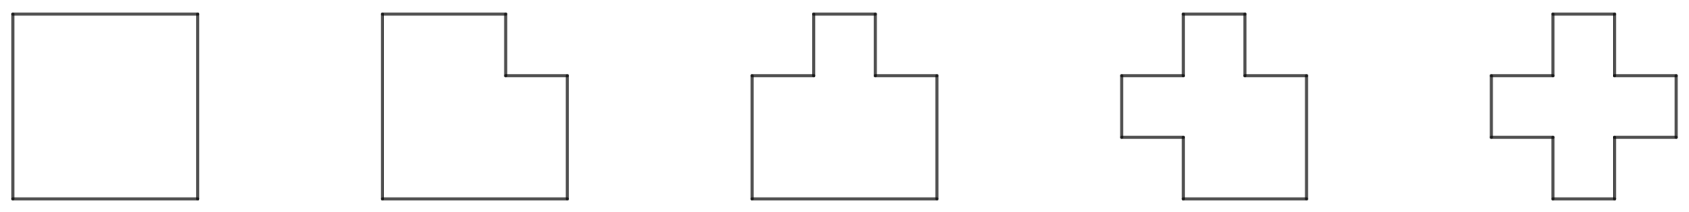
\includegraphics[width=.8 \paperwidth]{./images/EOrtogonales.png}
    \caption*{Ejemplos de polígonos ortogonales.}
  \end{figure}
\end{frame}

% Antecedente 1:
\begin{frame}{Antecedente I.} %%Otra forma (más corta) de poner el título a la diapositiva
  \framesubtitle{¿Cuántos vértices concavos hay en un polígono ortogonal?} %%Subtítulo de la diapositiva (opcional)
  Sabemos que los ángulos en un polígono ortogonal son $\frac{\pi}{2}$ o $\frac{3\pi}{2}$. Los vértices
  concavos son siempre de $\frac{3\pi}{2}$. \newline
  
  \textbf{Lema.} Todo polígono ortogonal con $n$ vértices tine
  $\frac{n - 4}{2}$
  vértices concavos.
  
  \begin{proof}
    Procedamos por inducción sobre el número de vértices. Es fácil ver que sólo podemos agregar $2m$ vértices
    a la vez, con $m \in \mathbb{Z}$. Supongamos que para $k$ vértices se cumple el lema. ¿Qué pasa con $k + 2$
    vértices?
    \[\frac{k - 4}{2} + 1 = \frac{k - 4 + 2}{2} = \frac{(k + 2) - 4}{2}.\]
  \end{proof}
\end{frame}

% Antecedente 2:
\begin{frame}{Antecedente II.} %%Otra forma (más corta) de poner el título a la diapositiva
  \framesubtitle{Clasificando vértices y aristas.} %%Subtítulo de la diapositiva (opcional)
  \begin{figure}
    \centering
    \begin{subfigure}[b]{0.4\paperwidth}
      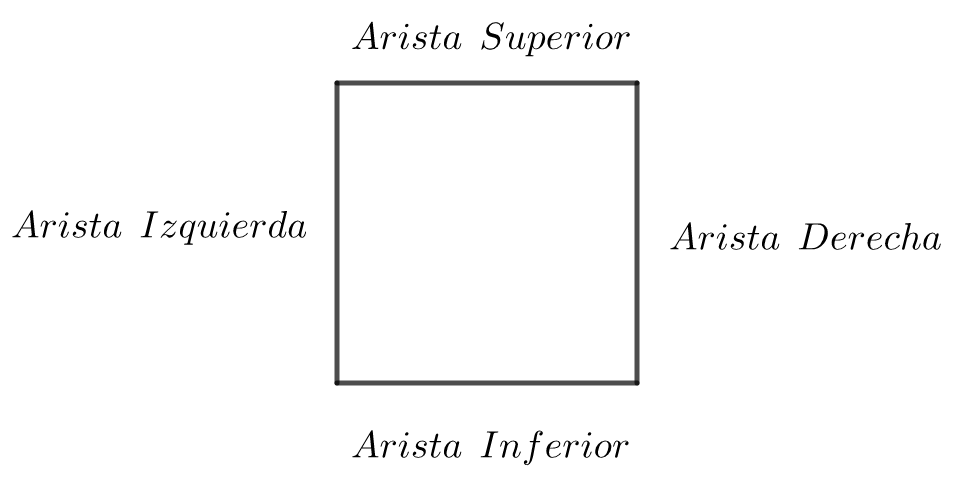
\includegraphics[width=0.4\paperwidth]{./images/CAristas.png}
      \caption*{Clasificación de aristas.}
    \end{subfigure}
        \begin{subfigure}[b]{0.4\paperwidth}
      \includegraphics[width=0.4\paperwidth]{./images/CVértices.png}
      \caption*{Clasificación de Vértices.}
    \end{subfigure}
  \end{figure}
\end{frame}

% Antecedente 3:
\begin{frame}{Antecedente III.} %%Otra forma (más corta) de poner el título a la diapositiva
  \framesubtitle{Clasificando vértices y aristas.} %%Subtítulo de la diapositiva (opcional)
  \begin{figure}
    \centering
    \includegraphics[width=0.8\paperwidth]{./images/Clasificación completa.png}
    \caption*{Clasificando aristas y vértices.}
  \end{figure}
\end{frame}

% Antecedente 4:
\begin{frame}{Antecedente IV.} %%Otra forma (más corta) de poner el título a la diapositiva
  \framesubtitle{Corte impar.} %%Subtítulo de la diapositiva (opcional)
  \textbf{Def.} Dado un polígono ortogonal $P$, definimos un \textit{corte horizontal} o \textit{vértical}
  de $P$, como la extensión de una arista horizontal o vértical de $P$ a partir de un vértice concávo hacia
  el interior de $P$ hasta un punto de intersección con la frontera de $P$.
  \begin{figure}
    \centering
    \begin{subfigure}[b]{0.2\paperwidth}
      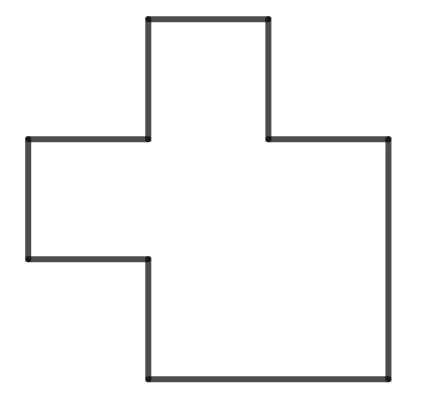
\includegraphics[width=0.1\paperwidth]{./images/Fig.png}
      \caption*{Polígono.}
    \end{subfigure}
    \begin{subfigure}[b]{0.2\paperwidth}
      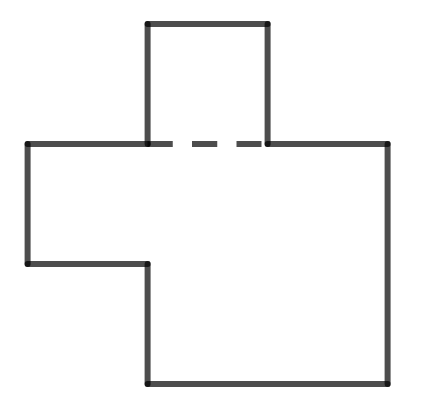
\includegraphics[width=0.1\paperwidth]{./images/FigCH.png}
      \caption*{Corte horizontal.}
    \end{subfigure}
    \begin{subfigure}[b]{0.2\paperwidth}
      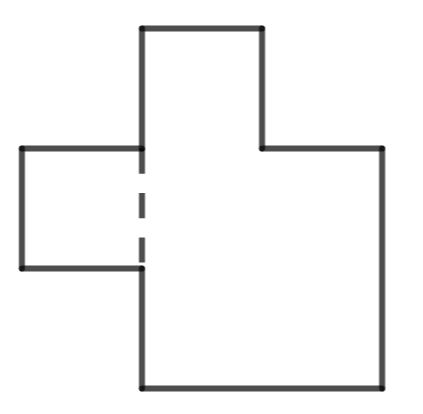
\includegraphics[width=0.1\paperwidth]{./images/FigCV.png}
      \caption*{Corte vértical.}
    \end{subfigure}
  \end{figure}
  \textbf{Def.} Un corte impar es un corte horizontal o vértical, tal que uno de los subpolígonos
  que forma es de tamaño $4k + 2$. Con $k \in \mathbb{Z}$.
\end{frame}
